\section{Predobrada podataka i izbor atributa}
\label{ch:ch3}

\subsection{Predobrada}
Za predobradu podataka korišten je programski jezik \textit{Python} u kombinaciji s paketom \textit{pandas}. Datoteka s podacima \textit{splice\_orig.csv} je učitana u \textit{pandas DataFrame} objekt te su dodani nazivi atributa: \textit{class}, \textit{id} i \textit{dna} (vidi tablicu \ref{tab:dataorig}).
\begin{table}[!ht]
   \caption[Primjeri instanci iz originalnog podataka]{
   \textbf{Primjeri instanci iz skupa podataka za dubinsku analizu.} \textit{}}
   \centering
   \begin{tabular}{||c | c | c ||}
   \hline
   class & id & dna \\ [0.5ex]
   \hline\hline
   EI & ATRINS-DONOR-905 & AGACCCGCCGGGAGGCGGAGGACCTGC... \\
   EI & BABAPOE-DONOR-30 & GAGGTGAAGGACGTCCTTCCCCAGGAG... \\
   EI & CHPIGECA-DONOR-378 & CAGACTGGGTGGACAACAAAACCTTCA... \\
   .. & .. & .. \\
   N & ORAHBG2F-NEG-181  & ATCAATAAGCTCCTAGTCCAGACGCCAT... \\
   N & ORARGIT-NEG-241 & TCTCGGGGGCGGCCGGCGCGGCGGGG... \\
   N & TARHBD-NEG-1981  & AGGCTGCCTATCAGAAGGTGGTGGCTG... \\ [1ex]
   \hline
   \end{tabular}
   \label{tab:dataorig}
\end{table}

Nakon što smo izbacili stupac \textit{id} i podijelili stupac \textit{dna} podaci imaju oblik kao u tablici \ref{tab:datasplit}.

\begin{table}[!ht]
   \caption[Primjeri instanci iz procesiranog skupa podataka]{
   \textbf{Primjeri instanci iz procesiranog skupa podataka za dubinsku analizu.} \textit{
Stupac \textit{id} je jedinstveni identifikator vrste za svaki red u tablici i zbog toga ga ne koristimo u analizi podataka. Stupac \textit{DNA} dijelimo na šezdeset stupaca, za svaki nukleotid u DNA nizu po jedan novi stupac, naziva dna\_x gdje x označava indeks nukleotida u originalnom nizu.
   }}
   \centering
   \begin{tabular}{||c | c | c |c | c | c | c ||}
   \hline
   class & dna{\_1} & dna{\_}2 & dna{\_}3\ & dna{\_}4\ & dna{\_}5 & ...\\ [0.5ex]
   \hline\hline
   EI & A & G & A & C & C & ... \\
   EI & G & A & G & G & T & ... \\
   EI & C & A & G & A & C & ... \\
   .. & .. & .. & .. & .. & .. & ... \\
   N & A  & T & C & A & A & ... \\
   N & T  & C & T & C & G & ... \\
   N & A  & G & G & C & T & ... \\ [1ex]
   \hline
   \end{tabular}
   \label{tab:datasplit}
\end{table}

\begin{table}[!ht]
   \caption[Udjeli nukleotida u skupu podataka za dubinsku analizu]{
   \textbf{Udjeli nukleotida u skupu podataka za dubinsku analizu.} \textit{A, G, C i T čine značajnu većinu u skupu podataka. D, N, S i R čine neznatan dio skupa.}}
   \centering
   \begin{tabular}{||c | c | c ||}
   \hline
   Oznaka atributa & Broj atributa & Udio atributa (\%) \\ [0.5ex]
   \hline\hline
   A & 44475 & 23.244 \\
   T & 46298 & 24.196 \\
   G & 50226 & 26.249 \\
   C & 50281 & 26.278 \\
   D & 2  & 0.0010 \\
   N & 56 & 0.0293 \\
   S & 1  & 0.0005 \\
   R & 1  & 0.0005 \\ [1ex]
   \hline
   \end{tabular}
   \label{tab:udjeli}
\end{table}
Razdiobe jedinstvenih oznaka nukleotida prikazane su u tablici \ref{tab:udjeli}. Vidimo da vrlo mali udio atributa ima oznaku D, N, S ili R (ukupno 15 redaka). Zbog toga možemo izbaciti ove retke bez značajnog smanjenja skupa podataka za dubinsku analizu. S druge strane, na ovaj način sprječavamo da algoritam daje previše važnosti podacima koji spadaju u ovu marginalnu skupinu (engl. \textit{outliers}). 
Jedna od instanci iz klase EI\footnote{HUMALPI1-DONOR} ima nukleotidni niz\textit{ 
ACACAGGGCACCCCCTCANNNNNNNNNNNNNNNNNNNNNNNNNNNNNNNNNNNNNNNNN
}. Čak 42 baze označene su s oznakom N. Ako bi svaki N zamijenili s jednom od četiri moguće baze dobili bismo 4\textsuperscript{42} kombinacija. Bez provjere u postojećim bazama podataka ne možemo znati koje su od tih kombinacija uistinu dijelovi donorskih sekcija u genomu. Korištenjem ovih kombinacija značajno bismo utjecali na distribuciju skupa podataka jer većina lokacija u genomima nije ni donorska ni akceptorska sekcija gena. Primjerice, u DNK molekuli čovjeka oko 27\% genoma čine sekvence koje se prepisuju u RNK, a od toga je samo oko 1.5\% kodirajućih sekvenci \cite{Berg01}.

Ovako obrađen skup podataka spremljen je u datoteku \textit{splice\_filtered.csv} za daljnju analizu.

\subsection{Skupovi podataka za treniranje i testiranje}

Prije nego krenemo s procesom obrade skup podataka dijelimo na dva dijela: skup za trening i skup za testiranje. Za testiranje izdvajamo 20\% od ukupnog skupa podataka i njih koristimo samo za završnu ocjenu odabranih modela. Želimo osigurati da su podaci stratificirani, odnosno da su razdiobe podataka jednake u ishodišnom skupu podataka kao i generiranim skupovima. 
\begin{center}
   \begin{figure}[ht!]
      \begin{center}
         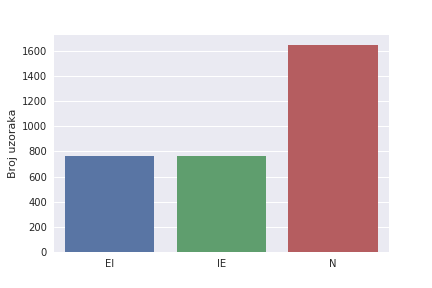
\includegraphics[height=6cm, width=9cm]{dataset_class_dist}
         \caption[Distribucija instanci u skupu podataka po klasama]
         {\textbf{Distribucija instanci u skupu podataka po klasama.} \textit{Prevladava klasa N, odnosno nizovi koji ne pripadaju ni akceptorskim ni donorskim nizovima nukleotida. U pojedinačnom genomu ova razlika je još izraženija \cite{Brown01} i kada bismo htjeli koristiti ovaj algoritam na drugim skupovima podataka morali bismo prilagoditi broj instanci odgovarajućim omjerima.}}
         \label{fig:dist_orig}
      \end{center}
   \end{figure}
\end{center}

Metoda \textit{test{\_}train{\_}split} iz paketa \textit{sklearn} ima argument \textit{stratify} kojem predajemo stupac s klasama. Slike \ref{fig:dist_orig} i \ref{fig:dist_train_test} potvrđuju da su podaci pravilno podijeljeni.

\begin{center}
   \begin{figure}[ht!]
   \begin{subfigure}{.5\textwidth}
         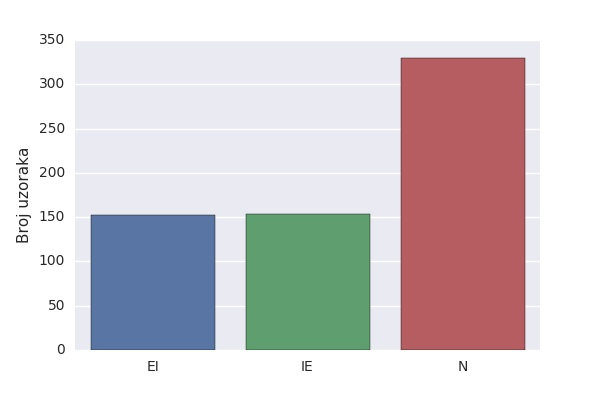
\includegraphics[height=5cm, width=8cm]{testset_class_dist}
         \caption{Trening}
         \label{fig:dist_train}
   \end{subfigure}
   \begin{subfigure}{.5\textwidth}
         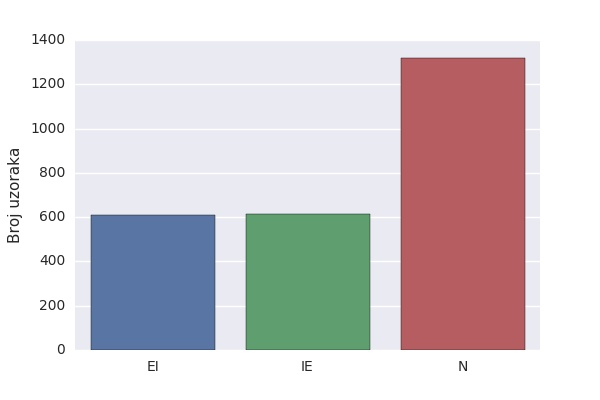
\includegraphics[height=5cm, width=8cm]{trainset_class_dist}
         \caption{Test}
         \label{fig:dist_test}
   \end{subfigure}
   \caption[Distribucija instanci u skupovima podataka za trening i test]
   {\textbf{Distribucija instanci u skupovima podataka za trening i test po klasama.} \textit{Vidimo da je distribucija skupa za trening (a) i skupa za testiranje (b) jednaka distribuciji izvornog skupa podataka. Razlika je samo ukupnom broju instanci u pojedinome skupu.}}
    \label{fig:dist_train_test}
   \end{figure}
\end{center}

\subsection{Odabir atributa}
Pri kreiranju modela za dubinsku analizu podataka obično nije nužno koristiti sve dostupne atribute skupa podataka. U odabiru najboljih atributa za model primjenjuju se različite tehnike koje se u grubo mogu svrstati u tri kategorije. Metode \textbf{filtriranja} najčešće koriste različite statističke testove kako bi se odredila korelacija\footnote{termin korelacija ovdje koristimo u širem smislu, ne isključivo u statističkom kontekstu} između atributa i izlazne varijable (klase). Druga kategorija, metode \textbf{omotača}\footnote{engl. \textit{wrapper methods}} koriste podskup atributa nad kojim treniraju model. Na osnovu zaključaka iz trenutnog modela, dodaju se ili oduzimaju određeni atributi - problem odabira atributa svodi se na problem pretraživanja. \textbf{Ugradbene} metode\footnote{engl. \textit{embedded methods}} kombiniraju kvalitete filterskih i metoda omotavanja korištenjem algoritama koji imaju vlastite ugrađene metode selekcije atributa.

Budući da su svi podaci u skupu nominalni, te da imamo veliki broj atributa, moguće ih je prikazati samo indirektnom mjerom ili parcijalno (slika \ref{fig:class_dna_x}).
\begin{center}
   \begin{figure}[ht!]
   \begin{subfigure}{.5\textwidth}
         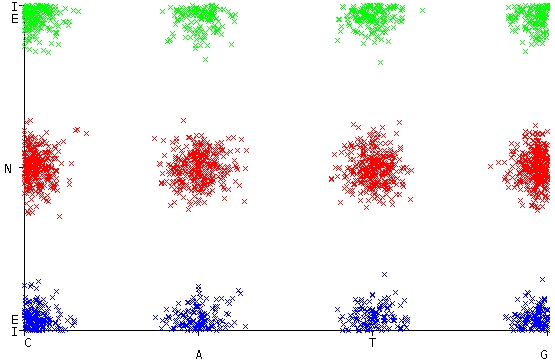
\includegraphics[height=5cm, width=8cm]{class_dna_2}
         \caption{dna{\_}2}
         \label{fig:class_dna_2}
   \end{subfigure}
   \begin{subfigure}{.5\textwidth}
         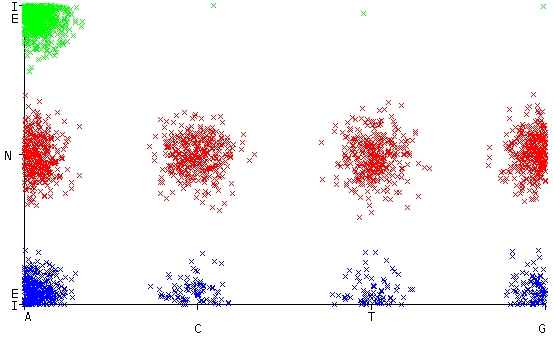
\includegraphics[height=5cm, width=8cm]{class_dna_29}
         \caption{dna{\_}29}
         \label{fig:class_dna_29}
   \end{subfigure}
   \begin{subfigure}{.5\textwidth}
         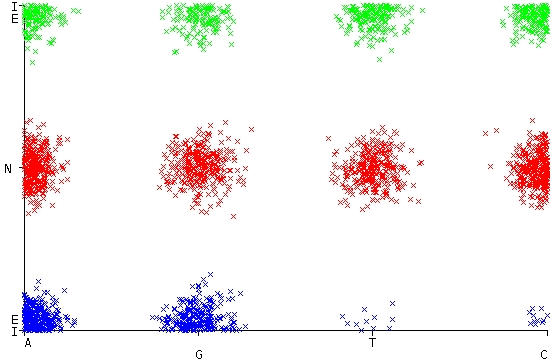
\includegraphics[height=5cm, width=8cm]{class_dna_33}
         \caption{dna{\_}33}
         \label{fig:class_dna_33}
   \end{subfigure}
   \begin{subfigure}{.5\textwidth}
         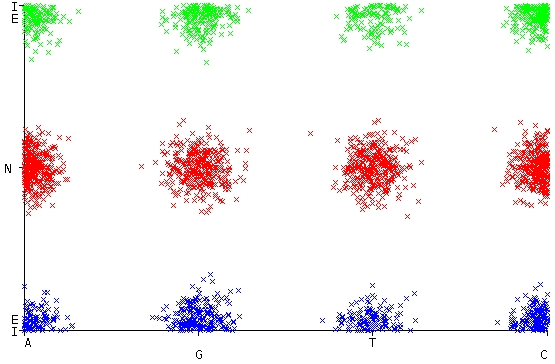
\includegraphics[height=5cm, width=8cm]{class_dna_54}
         \caption{dna{\_}54}
         \label{fig:class_dna_54}
   \end{subfigure}
   \caption[Dijagram rasipanja vrijednosti atributa po klasama]
   {\textbf{Frekvencija vrijednosti atributa po klasama.}\textit{ Distribucija vrijednosti atributa uniformna je na indeksima udaljenima od sredine nukleotidnog niza (\ref{fig:class_dna_2} i \ref{fig:class_dna_54}). Za indekse neposredno prije granice (\ref{fig:class_dna_29}) i poslije granice (\ref{fig:class_dna_33}) donorsko-akceptorskog područja vidimo da postoje izražena koncentracija određenih vrijednosti baza.}}
    \label{fig:class_dna_x}
   \end{figure}
\end{center}
Ovakva razdioba upućuje na zaključak da nisu svi atributi jednako značajni. Algoritam stabla odlučivanja (vidi poglavlje \ref{ch:ch4}) ima prirodno ugrađen mehanizam za odabir atributa. Najprije se u postupku konstrukcije rangiraju atributi, a zatim se u postupku podrezivanja smanjuje ukupan broj atributa. Neki računalni znanstvenici\cite{Grabczewski01} zbog ovih karakteristika koriste stablo odlučivanja kao algoritam za odabir atributa. Atributi izabrani na ovaj način zatim se koriste u drugome modelu koji može biti bilo klasifikacijski bilo regresijski postupak. U tom smislu, možemo promatrati stabla odlučivanja kao ugradbenu metodu odabira atributa. Budući da je procedura izgradnje stabla odlučivanja poprilično brza onda je moguće i koristiti sve atribute, a algoritam bi se u teoriji sam trebao pobrinuti da odabere najbolje atribute.
Kako bismo provjerili ovu hipotezu, kreirat ćemo i dodatne varijante stabla odlučivanja, nad podskupovima atributa. Kao metodu omotača koristimo odabir atributa pomoću višeslojnog perceptrona.
Budući da smo već utvrdili da postoji određena frekvencijska relacija vrijednosti atributa i klasa provodimo postupak selekcije atributa korištenjem prikladnog statističkog testa. Kao logičan postupak nameće se tzv. Hi-kvadrat test, koji možemo svrstati u skupinu filterskih metoda odabira atributa.
\subsubsection{Hi-Kvadrat test}
Hi-Kvadrat je test nezavisnosti koji se koristi kako bi se odredilo postoji li značajna veza između dvije nominalne (kategoričke) varijable. Frekvencija svake vrijednosti jedne nominalne varijable (atributa) uspoređuje se sa kategorijama druge nominalne varijable (klase). Računaju se očekivane vrijednosti frekvencija vrijednosti atributa i uspoređuju sa stvarnim vrijednostima iz skupa podataka. Podaci se prikazuju u kontigencijskim tablicama (tablica \ref{tab:contig}).
\begin{center}
    \begin{table}[!ht]
    \caption[Kontigencijska tablica]{
    \label{tab:contig}
    \textbf{Primjer kontigencijske tablice.} \textit{Stupci su kategorije jedne varijable (atributa), a redovi kategorije druge varijable (klase). Krajnji redak i stupac predstavljaju sumu vrijednosti iznad, odnosno lijevo. Na osnovu sumarnih vrijednosti računaju se očekivane vrijednosti kategorija.}}
   \centering
   \begin{tabular}{||c | c | c | c | c ||}
   \hline
     & Atr1 & ... & AtrN & SumA \\ [0.5ex]
   \hline\hline
   Klasa1 & $O_{11}$ & ... & $O_{1N}$ & $\sum_{j=1}^{N}O_{1j}$ \\
   ..     & ...    & $O_{mn}$ & ... & ... \\
   KlasaM & $O_{M1}$ & ... & $O_{MN}$ ... & ... \\ 
   \hline
   SumK & $\sum_{i=1}^{M}O_{i1}$ & ... & ... & $\sum_{i=1}^{M}\sum_{j=1}^{N}O_{ij}$ \\ [1ex]

    \hline
    \end{tabular}
    \end{table}
\end{center}
Najprije se računaju očekivane vrijednosti na osnovu tablice kontigencije korištenjem sljedeće formule

\begin{equation}\label{eq:chiexpect}
E_{ij} = \frac{\sum_{k=1}^{N}O_{ik}\sum_{k=1}^{M}O_{kj}}{N}
\end{equation}

gdje je 

\begin{itemize}
    \item $\sum_{k=1}^{N}O_{ik}$ - suma i-tog retka u kontigencijskoj tablici
    \item $\sum_{k=1}^{M}O_{kj}$ - suma j-tog stupca u kontigencijskoj tablici
    \item N - ukupan broj instanci u skupu podataka.
\end{itemize}

Nakon izračuna očekivanih vrijednosti, možemo se pristupiti izračunu vrijednosti Hi-kvadrat testa neovisnosti

\begin{equation}
    \chi^2 = \sum_{i=1}^{M}\sum_{j=1}^{N}\frac{(O_{ij}-E_{ij})^2}{E_{ij}}
\end{equation}

Hi-kvadrat testira određenu hipotezu čiju istinitost pretpostavljamo. Nulta hipoteza pretpostavlja da ne postoji statistički značajna veze između dvije varijable. Alternative hipoteza, pojednostavljeno, pretpostavlja suprotno od nulte hipoteze. Upotreba Hi-kvadrat testa detaljno je obrađena u \cite{Grubi01}.

Tablica \ref{tab:chi2} prikazuje primjer kontigencijske tablice za dva atributa, \textit{dna{\_2}} i \textit{dna{\_}29}, iz podataka nad kojima vršimo analizu. Odgovarajuća nulta i alternativna hipoteza mogu biti:
\begin{itemize}
    \item $H_0$: Nukleotid na n-tom indeksu nije povezan s klasom nukleotidnog niza, i 
    \item $H_1$: Nukleotid na n-tom indeksu povezan je s klasom nukleotidnog niza.
\end{itemize}

\begin{table}
\centering
    \caption[Sumarni podaci vrijednosti atributa za hi-kvadrat test]{\textbf{Sumarni podaci vrijednosti atributa za hi-kvadrat test.} \textit{Tablični pregled vrijednosti koje se koriste u hi-kvadrat testu za odabir atributa. Za atribut na indeksu 2 vidimo da se broj nukleotidnih baza poklapa sa distribucijom klasa u skupu. Za atribut na indeksu 29 vidimo da vrijednosti značajno odstupaju od razdiobe klasa.}}
    \label{tab:chi2}
    \csvautotabular{"data/chi2table.csv"}
\end{table}
Koristeći \eqref{eq:chiexpect} možemo izračunati da očekivana vrijednost kategorije T za atribut \textit{dna{\_}2} u slučaju klase IE iznosi $E_{IE2T} = 756*765/3174 = 182$ i razlika u odnosnu na stvarnu vrijednost je samo 14. U slučaju za atribut \textit{dna{\_}29} očekivana vrijednost na istoj poziciji u tablici iznosi $E_{IE29T} = 514*765/3174 = 124$, odnosno razlika je čak 123.

\subsubsection*{Weka chiSquaredAttributeEval}
Kako ne bismo morali ručno raditi izračun Hi-kvadrat vrijednosti cijelog seta koristimo modul \textit{chiSquaredAttributeEval} za selekciju atributa unutar Weka programskog alata. Ovaj paket nije u osnovnom instalacijskom paketu alata i treba ga naknadno instalirati korištenjem izbornika \textit{Tools->Package Manager} u početnom pregledniku programa \textit{Weka}. Postupak odabira je vrlo brz. Algoritam rangira atribute po kvaliteti te proizvoljno odlučujemo koliko ćemo parametara od toga odabrati za naš model. Kako bi smo povećali nepristranost postupka koristimo deseterostruku unakrsnu krosvalidaciju. Detalji korištenog modela s parametrima nalaze se u Dodatku A. 

\subsubsection{Višeslojni perceptron}
Višeslojni perceptron je tip neuronske mreže bez povratnih veza. Neuronska mreža (slika \ref{fig:mlp}) modelira razdiobu koja generira ulazni skup podataka $p_{model}(X)$.
\begin{figure}[!ht]
    \centering
    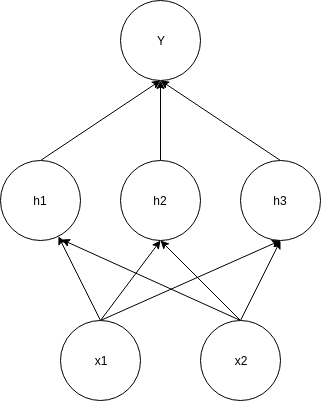
\includegraphics[height=6cm, width=5cm]{mlp}
    \caption[Model jednostavne neuronske mreže]{\textbf{Model jednostavne neuronske mreže.} \textit{$x_i$ su atributi instance koji čine ulazni sloj mreže, $h_i$ su neuroni skrivenog sloja, a $y$ je neuron u izlaznom sloju. Višeslojni perceptron mora imati minimalno ova tri sloja, a broj skrivenih slojeva u teoriji nije ograničen.}}
    \label{fig:mlp}
\end{figure}

Osnovna procesna jedinica u neuronskoj mreži je neuron, nazvan tako jer je modeliran prema stanicama živčanog sustava. Neuroni su u mreži organizirani u slojeve. Ulazni sloj prihvaća instancu kao ulazni podatak u obliku vektora atributa $X_N$. Neuron izračunava ponderiranu sumu atributa
\begin{equation}
    z = f(\textbf{x};\textbf{w},b) = \textbf{x}^T\textbf{w} + b
\end{equation}
gdje su $w$ parametri neurona, a b pomak (engl. \textbf{bias}). 
Nad rezultatom ove funkcije izračunava nelinearna transformacija, sigmoidna funkcija oblika
\begin{equation}
    y = \sigma(z) = \frac{1}{1+e^{-z}}
\end{equation}
ili $tanh(z)$. U posljednje vrijeme, najčešće se koristi ReLU\footnote{engl. \textit{Rectified Linear Unit}} aktivacijska funkcija.

Rezultat nelinearne transformacije iz svih neurona jednog sloja prosljeđuje se neuronima u sljedećem sloju. Završni sloj na izlazima daje vektor vjerojatnosti $Y_K$ da određena instanca pripada klasi $k$ korištenjem tzv. \textit{softmax} funkcije
\begin{equation}
    P(y=k|\textbf{x}) = \frac{e^{y_k}}{\sum_{i=1}^{K}e^{y_i}}
\end{equation}
Broj slojeva te broj neurona u sloju pripadaju tzv. hiperparametrima algoritma. Parametri mreže, tj. težine $W$ koje se koriste za izračun ponderirane sume uče se pomoću metode povratne propagacije greške. Stvarni izlazi mreže uspoređuju se sa željenim izlazima u svakom koraku učenja te se koristi odgovarajuća mjera pogreške. Metoda povratne propagacije određuje koliko trebamo prilagoditi parametre u pojedinim neuronima kako bi smo ovu grešku spustili na željenu razinu \cite{Goodfellow01}.

\subsubsection*{Weka MultilayerPerceptron}
Weka omogućava korištenje višeslojnog perceptrona u postupku odabira atributa. Koristi se modul \textit{ClassifierSubsetEval} unutar kojeg se podešava algoritam za selekciju \textit{classifiers.functions.MultiLayerPerceptron}. Postupak treniranja mreže za odabir traje oko tri sata na računalu s IntelCore i5 procesorom i 8GB RAM memorije. Treniranje modela izvršeno je nad cjelokupnim trening setom. Ovaj model izabrao je ukupno trinaest atributa. Detalji modela s korištenim parametrima nalaze se u dodatku A.
